% !TEX root =  paper.tex

\section{Background and Motivation}
\label{sec:motivation}


\subsection{The internals of modern crawlers}
\label{sec:background-crawlers}

\Cref{fig:abstract-crawler} illustrates the architecture of an abstract crawler
tailored for modern web apps.
The crawler starts by exploring the web app under analysis
from a starting point, e.g., the URL pointing to the web app's first page.
The crawler navigates a web browser to that URL,
and then extracts actionables in the loaded page.
These are DOM elements that the crawler could interact with
to change the \textit{state} of the application.
These elements are \textit{candidate} actionables
for a crawler, since it does not know whether interacting with them will 
lead to a new state a priori.
Subsequently, the crawler chooses the next event corresponding to a candidate actionable,
fires it,
and monitors the web browser to see whether there is a change in the current state of the web app.

Crawlers often allow custom \textit{state abstraction function}s; i.e.,
definitions for what constitutes a web app state
(e.g., a DOM snapshot, or a screenshot of the web page).
The crawler then chooses the next state to \textit{expand}
(i.e., to identify actionables on that state and continue the crawling from there)
based on a \textit{state exploration strategy}.
While crawling, the crawler can construct a model of the web app under analysis
using the states and transitions between them.
This can be a graph where each node is a state, 
and each edge is the event that caused the following state to be explored
(i.e., the \textit{state-flow graph}~\cite{Mesbah:2012:Crawljax}).
This model is then used for different purposes,
e.g., automated test case generation~\cite{Mirshokrae:2015:JSFeet}.

\begin{figure}
	\centering
	\includegraphics[width=\linewidth]{figures/crawler-internals}
	\caption{The internals of an abstract crawler.}
	\label{fig:abstract-crawler}
\end{figure}


\begin{figure}[h]
	\centering
	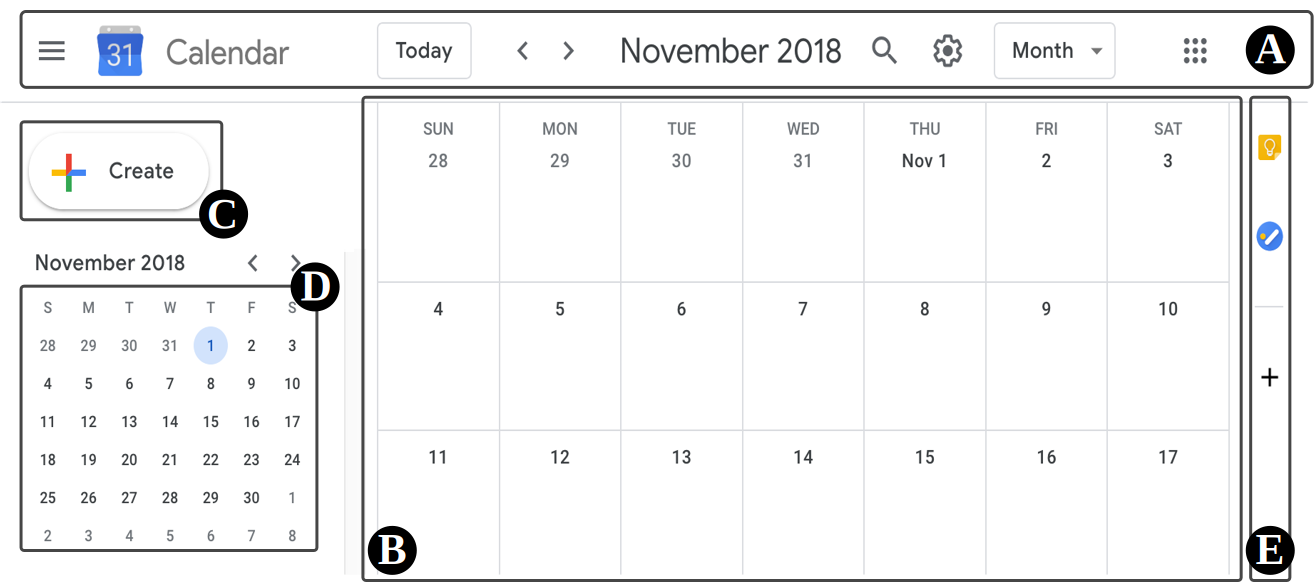
\includegraphics[width=\linewidth]{figures/motivating-example}
	\caption{Interactive elements on Google Calendar's web UI.}
	\label{fig:motivating-example}
\end{figure}

\subsection{Motivating example}
\label{sec:motivating-example}

\Cref{fig:motivating-example} depicts a screenshot of Google Calendar, 
a highly-dynamic modern web app.
If we were to use an automated crawler to analyze Google Calendar
we would observe the following:



%\begin{enumerate}[leftmargin=*]

	 
\header{Actionables}
	There is a large set of actionable elements that are candidates for interacting with
	to cover different functionalities.
	The \textit{actionables extractor} component of the crawler
	(i.e., the shaded box in \Cref{fig:abstract-crawler}) is responsible for identifying these elements.
	Most of these elements in Google Calendar are \code{<div>}s and not hyperlinks (i.e., \code{<a>} tags).
	This includes, for example, all elements in groups \circled{A}, \circled{B}, \circled{D} and  \circled{E} in \Cref{fig:motivating-example}. 
%	Indeed, prior research has revealed that hyperlinks are not the main element type to reach the hidden states of web applications~\cite{Behfarshad:2013:HiddenWeb}.
	Most web crawlers focus on hyperlinks and miss a large portion of actionables to be fired~\cite{Andreasen:2017:SurveyOfDynamicAnalysis}.
	More advanced crawlers~\cite{Mesbah:2012:Crawljax} give the user the option to specify the type of web elements (e.g., \code{div}) to consider as candidate actionables, which is still not ideal as the user has to manually configure the crawler.
	%of aiding the crawler 
%	by manually configuring which specific \code{<div>} elements to examine
%	(e.g., using XPath or \css locators).
	
	Our goal in this work is to devise a technique that predicts \textit{a priori} which elements on a page are actionables, %event listeners attached to the elements
	%to reach a higher coverage 
	regardless of their element type and without manual configuration.
	
	\header{Equivalent classes of actionables} There are usually equivalent classes of actionables
	that appear within or across different states,
	and share similar functionality.  
%	in the associated \js code, 
%	so that triggering similar user events on them would initiate almost identical functionality.
	For instance, in Google Calendar, clicking on any of the displayed \textit{days} 
	(i.e., elements in group \circled{B} or \circled{D} in \Cref{fig:motivating-example})
	would result in seeing the calendar events corresponding to the selected day (elements in \circled{D}),
	or creating new calendar event in the selected day (elements in \circled{B}).
	%Crawlers find new states by clicking on the elements in the page. 
	In such cases where the corresponding functionalities are similar (or identical), 
	 firing events on these similar actionables is unlikely to result in new states
	or more \js code coverage.
	This can bear several implications in practice.
	If, for example, the crawler is configured to run within a certain time limit (which is the usual case in practice),
	it is highly probable that it would waste some of its runtime on those equivalent actionables. 
	In our motivating example of \Cref{fig:motivating-example}, 
	a more intelligent mechanism would be to 
	avoid firing events on the actionables in groups \circled{B} and \circled{D} again, 
	and moving on to another part of the web app,
	e.g., elements in groups \circled{A}, \circled{C}, or \circled{E} 
	which are likely to yield more different states and also cover a broader range of \js code.

	
%\end{enumerate}


